\documentclass[answers]{exam}

\usepackage[dvipsnames]{xcolor}
\usepackage{amsmath}
\usepackage{amsfonts}
\usepackage{amsthm}
\usepackage{microtype}
\usepackage{siunitx}
\DeclareSIUnit\year{yr}
\usepackage{pgfplots}
\usepackage{graphicx}
\usepackage{sidecap}
\sidecaptionvpos{figure}{c}
\usepackage{float}
\usepackage{hyperref}
\usepackage{gensymb}
\usepackage{tkz-euclide}
\usetkzobj{all}
\usepackage{commath}
\usepackage{steinmetz}

\newtheorem*{thm}{Theorem}

% russian integral
\usepackage{scalerel}
\DeclareMathOperator*{\rint}{\scalerel*{\rotatebox{17}{$\!\int\!$}}{\int}}

% \qformat{Question \thequestion: \thequestiontitle\hfill}

\begin{document}

\section*{NCEA Level 3 Trigonometry (exercise set)\\5. The Sine and Cosine Laws}
\paragraph{Goal} To consider the relations of arbitrary (i.e. non-right-angled) triangles and associated circles.

\begin{questions}
  \question There exists a point $ O $ inside the regular tetrahedron $ ABCD $ such that $ O $ is equidistant from
            the four vertices. (You may assume this without proof.) Compute the angle between $ OA $ and $ OB $.
            \begin{center}
              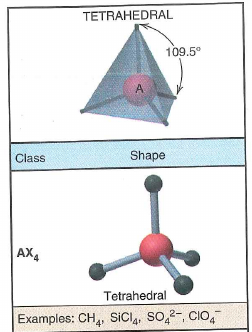
\includegraphics[width=0.2\textwidth]{exercises-5-3}
            \end{center}
            (Image credit: Silberberg, \textit{Chemistry} 3e, figure 10.8.)
  \question The proof of the cosine rule, as given in the notes, only works if $ c \leq a $ (i.e. if the chords intersect
            inside the circle). Show that if $ c > a $ then the same idea works (consider exercise 5.3).
  \question
    \begin{parts}
      \part Let $ A $ and $ B $ be two points. Show that the set of all points equidistant from $ A $ and $ B $ is just the
            line perpendicular to the segment $ AB $, that passes through the midpoint of $ A $ and $ B $.
      \part The circumcentre (centre of the circumcircle) of a triangle $ ABC $ is the point equidistant from all three vertices.
            Show that the circumcentre is the point of intersection of the perpendicular bisectors of the sides of the triangle (so
            in particular all three lines pass through a single point).
      \part Suppose $ ABC $ is a triangle. Show that there exists a (unique) circle with centre inside $ ABC $ that touches
            each side of $ ABC $ precisely once (i.e. it is tangent to each side).
            \begin{center}
              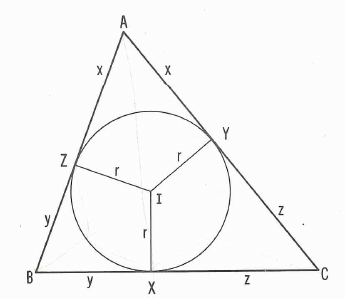
\includegraphics[width=0.3\textwidth]{exercises-5-1}
            \end{center}
            (Image credit: Coxeter, \textit{Geom. Revisited}, figure 1.4A.) Hints:
        \begin{subparts}
          \subpart Draw the triangle $ ABC $.
          \subpart Suppose the angle at $ A $ has measure $ \alpha $; draw the line through $ A $ that bisects the angle there (i.e. cuts
                   it into two angles of measure $ \alpha/2 $). Likewise, draw angle bisector lines through $ B $ and $ C $.
          \subpart Show that, if $ P $ is on the angle bisector line through the vertex $ A $, then $ P $ is equidistant from $ AB $ and $ AC $.
                   (The distance from a point $ P $ to a line $ \ell $ is the length of the segment with one end $ P $ and
                   perpendicular to $ \ell $ at the other end.)
          \subpart Use (iii) and a similar argument to (b) above to show that all three bisectors intersect at a single point $ O $ that
                   is equidistant to all three sides.
        \end{subparts}
    \end{parts}
  \clearpage
  \question Prove the \emph{Steiner-Lehmus theorem}: if a triangle has two equal angle bisectors (see 2(c)(ii) above), then it is isoceles.

            ``This theorem was sent to the great Swiss geometer Jacob Steiner in 1840 by C. L. Lehmus (whose name would otherwise have been forgotten
            long ago) with a respect for a pure geometrical proof. Steiner gave a fairly complicated proof which inspired many other people to look
            for simpler methods. Papers on the Steiner-Lehmus theorem appeared in various journals in 1842, 1844, 1848, almost every year from 1854 till
            1864, and with a good deal of regularity during the next hundred years.'' (Coxeter and Greitzer, \textit{Geometry Revisited}, \S1.5. Random House (1967).)

            Remark: This may be the most difficult exercise in any of the exercise sets for this topic. However, I will not give
            any hints because there are multiple productive avenues of study for you. A number of solutions are given in the paper linked
            in the footnote, and a purely geometric one is given in the citation for the above quote.\footnote{R\'obert~Ol\'ah-G'al and J\'ozsef~S\'andor,
            \textit{On Trigonometric Proofs of the Steiner-Lehmus Theorem}. Forum Geometricorum, Volume 9 (2009) 155–160.
            \url{http://forumgeom.fau.edu/FG2009volume9/FG200914.pdf}. See also \url{https://cs.nyu.edu/pipermail/fom/2004-August/008394.html} for
            a philosophical reason that no `easy' proof exists.}
\end{questions}

\paragraph{Additional reading} Coxeter, \textit{Intro. to Geometry}, sections 1.4 to 1.6 inclusive. Coxeter, \textit{Geometry Revisited}, chapter 1.

\end{document}
